\documentclass{article}

\usepackage{graphicx}
\usepackage{listings}

%http://tex.stackexchange.com/questions/140567/drawing-karnaughs-maps-in-latex
\usepackage{tikz}
\usetikzlibrary{matrix,calc}
%internal group
%#1 - Optional. Space between node and grouping line. Default=0
%#2 - top left node
%#3 - bottom right node
%#4 - filling color
\newcommand{\implicant}[4][0]{
	\draw[rounded corners=3pt, fill=#4, opacity=0.3] ($(#2.north west)+(135:#1)$) rectangle ($(#3.south east)+(-45:#1)$);
}

%Empty Karnaugh map 2x4
\newenvironment{Karnaugh}%
{
\begin{tikzpicture}[baseline=(current bounding box.north),scale=0.8]
\draw (0,0) grid (4,2);
\draw (0,2) -- node [pos=0.7,above right,anchor=south west] {$Q_1Q_0$} node [pos=0.7,below left,anchor=north east] {$Q_2$} ++(135:1);
%
\matrix (mapa) [matrix of nodes,
        column sep={0.8cm,between origins},
        row sep={0.8cm,between origins},
        every node/.style={minimum size=0.3mm},
        anchor=4.center,
        ampersand replacement=\&] at (0.5,0.5)
{
                      \& |(c00)| 00         \& |(c01)| 01         \& |(c11)| 11         \& |(c10)| 10         \& |(cf)| \phantom{00} \\
|(r00)| 0             \& |(0)|  \phantom{0} \& |(1)|  \phantom{0} \& |(3)|  \phantom{0} \& |(2)|  \phantom{0} \&                     \\
|(r01)| 1             \& |(4)|  \phantom{0} \& |(5)|  \phantom{0} \& |(7)|  \phantom{0} \& |(6)|  \phantom{0} \&                     \\
|(rf) | \phantom{00}  \&                    \&                    \&                    \&                    \&                     \\
};
}%
{
\end{tikzpicture}
}

%Places 1 in listed positions
\newcommand{\minterms}[1]{%
	\foreach \x in {#1}
		\path (\x) node {1};
}

%Places 0 in listed positions
\newcommand{\maxterms}[1]{%
	\foreach \x in {#1}
		\path (\x) node {0};
}

\title{Homework 5}
\author{Mitchel Fields}
\begin{document}

\maketitle

\begin{itemize}
	\item [\textbf{Part 1}]\hspace{0pt}\\

	\begin{tabular}{c | c}
	$S_n$ & $S_{n+1}$ \\ \hline
	$S_0$ & $S_1$ \\
	$S_1$ & $S_2$ \\
	$S_2$ & $S_3$ \\
	$S_3$ & $S_4$ \\
	$S_4$ & $S_5$ \\
	$S_5$ & $S_2$ \\
	$S_6$ & $S_7$ \\
	$S_7$ & $S_6$
	\end{tabular}

	8 states means 3 bits.
	
	\begin{tabular}{c | c}
	$S_n$ & $S_{n+1}$ \\ \hline
	$S_0$ & 110 \\
	$S_1$ & 100 \\
	$S_2$ & 000 \\
	$S_3$ & 001 \\
	$S_4$ & 011 \\
	$S_5$ & 010 \\
	$S_6$ & 101 \\
	$S_7$ & 111
	\end{tabular}

	\begin{tabular}{c c c | c c c}
	$Q^n_2$ & $Q^n_1$ & $Q^n_0$ & $Q^{n+1}_2$ & $Q^{n+1}_1$ & $Q^{n+1}_0$ \\ \hline
	$1$ & $1$ & $0$ & $1$ & $0$ & $0$ \\
	$1$ & $0$ & $0$ & $0$ & $0$ & $0$ \\
	$0$ & $0$ & $0$ & $0$ & $0$ & $1$ \\
	$0$ & $0$ & $1$ & $0$ & $1$ & $1$ \\
	$0$ & $1$ & $1$ & $0$ & $1$ & $0$ \\
	$0$ & $1$ & $0$ & $0$ & $0$ & $0$ \\
	$1$ & $0$ & $1$ & $1$ & $1$ & $1$ \\
	$1$ & $1$ & $1$ & $1$ & $0$ & $1$
	\end{tabular}

	$D_2 = Q_2(Q_1 + Q_0)$\\
	$D_1 = Q_0(\overline{Q_1} + \overline{Q_2})$\\
	$D_0 = \overline{Q_2}.\overline{Q_1} + Q_2Q_0$

	\begin{tabular}{c c c | c c c}
	$Q^n_2$ & $Q^n_1$ & $Q^n_0$ & R & Y & G \\ \hline
	$1$ & $1$ & $0$ & $1$ & $0$ & $0$ \\
	$1$ & $0$ & $0$ & $1$ & $0$ & $0$ \\
	$0$ & $0$ & $0$ & $0$ & $0$ & $1$ \\
	$0$ & $0$ & $1$ & $0$ & $1$ & $0$ \\
	$0$ & $1$ & $1$ & $1$ & $0$ & $0$ \\
	$0$ & $1$ & $0$ & $1$ & $1$ & $0$ \\
	$1$ & $0$ & $1$ & $0$ & $0$ & $0$ \\
	$1$ & $1$ & $1$ & $1$ & $0$ & $0$
	\end{tabular}\\

	Python simulation:

	\lstinputlisting[language=Python]{homework5.py}

	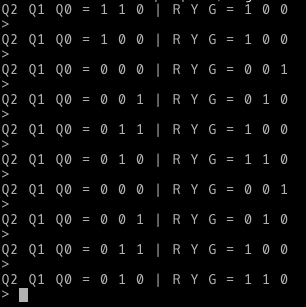
\includegraphics{hw5a}\\
	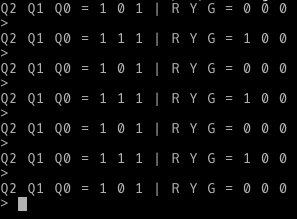
\includegraphics{hw5b}\\

	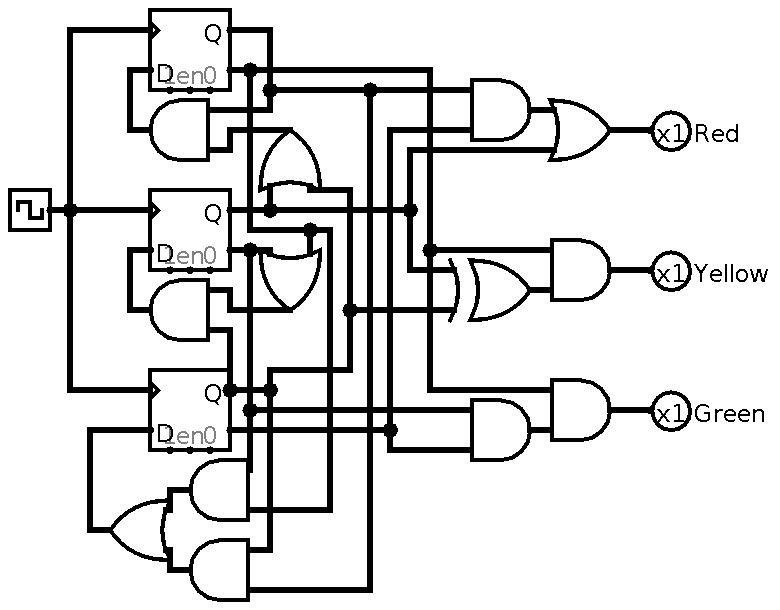
\includegraphics[scale=0.5]{hw5-1}

	\item [\textbf{Part 2}]\hspace{0pt}\\
	There are 4 ways to connect $S_6$ or $S_7$ to another state by changing only one bit: $101 \rightarrow 100$, $101 \rightarrow 001$, $111 \rightarrow 110$, and $111 \rightarrow 011$\\
	Of these options, only $101 \rightarrow 001$ reduces the number of covers in a Karnaugh map of the affected bits.\\

	\large{$D_2$}
	\begin{Karnaugh}
		\maxterms{0,1,2,3,4}
		\minterms{5,6,7}
		\implicant{7}{6}{red}
		\implicant{5}{7}{blue}
	\end{Karnaugh}

	Becomes:

	\large{$D_2$}
	\begin{Karnaugh}
		\maxterms{0,1,2,3,4,5}
		\minterms{6,7}
		\implicant{7}{6}{blue}
	\end{Karnaugh}

	The result changes the equation for $D_2$ from $D_2 = Q_2(Q_1 + Q_0)$ to $D_2 = Q_2Q_1$. The adjusted circuit diagram is as follows:\\

	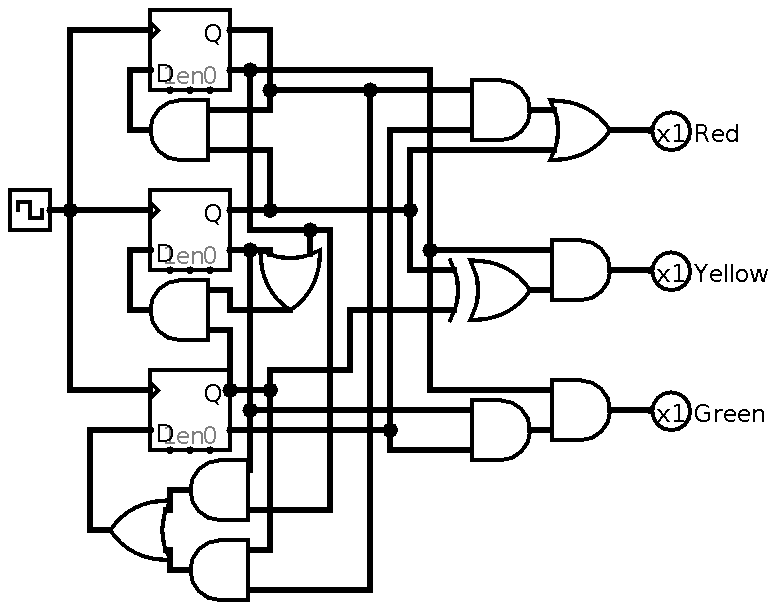
\includegraphics[scale=0.5]{hw5-2}

\end{itemize}

\end{document}